

\input{../Latex_Templates/Preamble_Report}

%%%%% TITLE PAGE

%\subject{, VT23}
\title{ Report for the Course Modelling in Computational Science, HT23 \\[1ex]
	  \large Project 1: The Potts model}
%\subtitle{}
\author{Theo Koppenhöfer \\[1ex] Group 4 (Anna Rockstroh, Carmen Lopez)}
\date{Lund \\[1ex] \today}

\addbibresource{bibliography.bib}

\usepackage{pythonhighlight}
\usepackage{pgfplots}
\graphicspath{{../Figures/}}

\pgfplotsset{
	compat=newest,
    every axis/.append style={
        axis y line=left,
        axis x line=bottom,
        scale only axis,
%    	max space between ticks=25pt,
        width=0.7\textwidth,
        scaled ticks=true,
        axis line style={thick,-,>=latex, shorten >=-.4cm},
    		x tick label style={
		    /pgf/number format/precision=3
		}
    },
    every axis plot/.append style={thick},
    tick style={black, thick}
}

%%%%% The content starts here %%%%%%%%%%%%%


\begin{document}

\maketitle

\section{Introduction}

The following report is part of the first project of the Modelling in Computational Science course at Lund University, HT2023.
In this project we implemented a Monte-Carlo simulation of the $q$-state Potts model. In the first part of this report we will describe the Potts model, the Monte-Carlo algorithms and some technicalities regarding the implementation. In the second part we will describe several experiments and the results they yielded. The main source for the report were \cite{AndersIrsb} and  \cite{AndersIrsb2}.
The report and the Python implementation can be found online under \cite{Repository}.

\section{The setup}

\subsection{The Potts model}

The following is a brief introduction to the Potts model from statistical mechanics which describes the spin of a particle on a grid.
A state of the $q$-state Potts model of a $L\times L$ flat grid is given by a mapping from the grid points to the spin states
\begin{align*}
	s\colon \brk[c]{1,\dots,L}\times\brk[c]{1,\dots,L}\to\brk[c]{1,\dots,q}\,.
\end{align*}
One assigns this state an energy via
\begin{align*}
	E(s) = -J\sum_{\substack{i, j\text{ neighbouring}\\ \text{grid points}}}\delta\brk*{s_i,s_j}
\end{align*}
where $\delta$ denotes the Kronecker-delta and $J=1$ is the coupling strength. As given in the problem setting we assume periodic boundary conditions on the grid. The aim is to evaluate the integral
\begin{align}
	\brk[a]*{E} = \int E(s)p(s) \dif s\,.\label{eq:integralAim}
\end{align}
Here $p$ is the density corresponding to the Boltzmann distribution, i.e.\
\begin{align*}
	p(s) = \frac{\exp\brk*{-E(s)/T}}{Z}
\end{align*}
with $Z$ a normalisation constant and $T$ the temperature. To evaluate the integral in \eqref{eq:integralAim} we will use random sampling of $s$ with the samples distributed according to the Boltzmann distribution. In other words, we will use a Monte-Carlo simulation.

\subsection{The Monte-Carlo algorithms}

To determine the statistical behaviour of the Potts model we use Monte-Carlo simulations. 
The first method we implemented was the Metropolis algorithm.
The steps for the Metropolis algorithm are given in figure \ref{alg:Metropolis}. A single iteration of this algorithm is performed by the function \pyth{MC_step_fast} in the implementation. In the implementation we used the pseudo-random number generators from \pyth{numpy.random} for the proposed spins, spin states and for determining if the choice should be accepted. For more information on the Metropolis Monte-Carlo simulation and the Potts model see \cite{AndersIrsb}.

\begin{figure}
\centering
\begin{algorithm}[H]
\caption{Metropolis}
\label{alg:Metropolis}
\SetKwInOut{Input}{Input}

\Input{Initial data $s$, $L$, $T$, $q$}
\BlankLine
\For{$k=0,1,\dots$}{
	Pick a point on the grid.
	
	Propose a new random spin value for this point.
	
	Calculate the change of energy $\Delta E$ that this spin flip would cause.
	
	Accept this spin flip with probability $\min\brk[c]*{1,\exp(-\Delta E/T)}$.
}
\end{algorithm}
\end{figure}

Analogously to the Metropolis algorithm the steps of the heat-bath algorithm are given in figure \ref{alg:heat-bath}. Its step differs from the Metropolis algorithm only after a point on the grid was randomly chosen. In the implementation a single iteration is performed by the function \pyth{Gibbs_step}. In the implementation for this algorithm we also used the \pyth{numpy.random} functions. For more details on the heat-bath algorithm see e.g.\  \cite{AndersIrsb2}.

\begin{figure}
\centering
\begin{algorithm}[H]
\caption{Heat-bath}
\label{alg:heat-bath}
\SetKwInOut{Input}{Input}

\Input{Initial data $s$, $L$, $T$, $q$}
\BlankLine
\For{$k=0,1,\dots$}{
	Pick a point on the grid.
	
	Pick a spin value for this point with a probability given by the distribution
	\begin{align*}
		p(s_i) = C \exp\brk*{\frac{1}{T}\sum_{j\text{ neighbours }i}\delta\brk*{s_i,s_j}}\,.
	\end{align*}
	Here $C$ is a normalisation constant.
}
\end{algorithm}
\end{figure}

\subsection{Some implementation details}

\subsubsection{Determining when the Energy has plateaued}

In order for the simulation to start sampling we needed a criteria to determine the time $t_0$ when the system reaches an equilibrium state.
 To determine $t_0$ we calculate in every step $i$ moving averages $\text{ma}_1$ and $\text{ma}_2$ over $n$ energies. The construction is shown in figure \ref{fi:movingAverages}. If we start in the hot state then the energy will tend to decrease until we reach an equilibrium. Hence we can use the condition
\begin{align}
	\text{ma}_2 \leq \text{ma}_1 \label{eq:equilCondition}
\end{align}
to determine $t_0$. If on the other hand we start in cold state the energy will in general increase and we have to reverse the inequality in equation \eqref{eq:equilCondition}. After reaching an equilibrium the simulation runs for a further \pyth{M_sampling} steps. It is over these samples we take the mean and the standard deviation.

\begin{figure}
\centering
\input{../Figures/explanationMovingAverages.pdf_tex}
\caption{A visualisation of the moving averages.}
\label{fi:movingAverages}
\end{figure}

\subsubsection{Improving performance}

While simulating we run into performance issues due to the fact that Python is in general rather slow even with heavy use of \pyth{numpy}. We resolved this issue with the help of \pyth{numba} which precompiles functions and thus increased performance substantially. The downside is that the code becomes quite unaesthetic because \pyth{numba} does not support all \pyth{python} and \pyth{numpy} features. In hindsight it would probably been better to have written the iteration in a language other than python.
In the experiments we also preferred to use the Metropolis algorithm because our implementation of this algorithm ran faster than the heat-bath algorithm.

\section{The experiments}

\subsection{A brief sanity check}

In order to check that our code was indeed doing what it was supposed to we designed some sanity checks. 
The energy during the simulation is updated with the calculated value for $\Delta E$.
Hence we checked with the function \pyth{test_energies} if the energy of the end state of the simulation is the same as the energy calculated during the simulation. Indeed, the last time I checked this was the case.

We also ran the simulation for both the Metropolis and the heat-bath algorithms and for a hot start and a cold start and compared the results. In the hot start the state $s$ is randomly initialised and in the cold start $s$ is initialised to have a constant value. We set the parameter $q=2$ and the grid size to $L=100$. In a first experiment the temperature was set to $T=100$. The result for the energies per spin is plotted in figure \ref{pl:HC_test_warm}. One can see that for both initialisations and for both algorithms the energy converges to a fixed value close to $-1$. Since the temperature is relatively `hot' the hot start reaches equilibrium faster than the cold start. The energy per spin value of almost $-1$ means that two neighbouring points will almost surely differ in their spin as would be expected for hot temperatures.
In a second experiment the temperature was set to $T=0.1$ and the result can be seen in figure \ref{pl:HC_test_cold}. Here too the energies per spin start to converge to a fixed lower value close to $-2$ but for the hot starts this process takes far longer. The energy per spin value of almost $-2$ means that two given neighbouring points will almost surely agree in their spins. This should be expected for cold temperatures.


\begin{figure}
\centering
\begin{minipage}{0.7\textwidth}
\centering
\graphicspath{{../../Plots/}}
\input{../../Plots/Hot-cold-starts_100.0_2.pgf}
\caption{Energy evolution for the temperature $T=100$}
\label{pl:HC_test_warm}
\end{minipage}
\end{figure}

\begin{figure}
\centering
\begin{minipage}{0.7\textwidth}
\centering
\graphicspath{{../../Plots/}}
\input{../../Plots/Hot-cold-starts_0.1_2.pgf}
\caption{Energy evolution for the temperature $T=0.1$}
\label{pl:HC_test_cold}
\end{minipage}
\end{figure}

\subsection{State plots}

We also plotted the state of the system for a system size $L=20$ with parameter $q=5$ after $M=10^4$ iterations for the temperatures $T=0.1$, $T=1$ and $T=100$. Figure  \ref{fi:Low_temp_state} shows the state for the low temperature, figure  \ref{fi:Medium_temp_state} for the medium temperature and figure \ref{fi:High_temp_state} for the high temperature.
We can see that as the temperature increases the state of the system gradually becomes more chaotic. For low temperatures there are larger patches of the same state. This corresponds to a lower energy configuration. In the implementation one can also see an animated version of the evolution of the system state for the different temperatures.

\begin{figure}
\begin{minipage}{0.3\textwidth}
\centering
\graphicspath{{../../Plots/}}
% This file was created with tikzplotlib v0.10.1.
\begin{tikzpicture}

\definecolor{lightgray}{RGB}{211,211,211}

\begin{axis}[
tick align=outside,
tick pos=left,
x grid style={lightgray},
xmajorgrids,
xmin=-0.5, xmax=19.5,
xtick style={color=black},
y dir=reverse,
y grid style={lightgray},
ymajorgrids,
ymin=-0.5, ymax=19.5,
ytick style={color=black}
]
\addplot graphics [includegraphics cmd=\pgfimage,xmin=-0.5, xmax=19.5, ymin=19.5, ymax=-0.5] {../../Plots/Low_temp_state_10000-002.png};
\end{axis}

\end{tikzpicture}

\caption{State for temperature $T=0.1$.}
\label{fi:Low_temp_state}
\end{minipage}
\hfill
\begin{minipage}{0.3\textwidth}
\centering
\graphicspath{{../../Plots/}}
% This file was created with tikzplotlib v0.10.1.
\begin{tikzpicture}

\definecolor{darkgray176}{RGB}{176,176,176}

\begin{axis}[
tick align=outside,
tick pos=left,
x grid style={darkgray176},
xmin=-0.5, xmax=19.5,
xtick style={color=black},
y dir=reverse,
y grid style={darkgray176},
ymin=-0.5, ymax=19.5,
ytick style={color=black}
]
\addplot graphics [includegraphics cmd=\pgfimage,xmin=-0.5, xmax=19.5, ymin=19.5, ymax=-0.5] {../../Plots/Medium_temp_state_10000-000.png};
\end{axis}

\end{tikzpicture}

\caption{State for temperature $T=1$.}
\label{fi:Medium_temp_state}
\end{minipage}
\hfill
\begin{minipage}{0.3\textwidth}
\centering
\graphicspath{{../../Plots/}}
% This file was created with tikzplotlib v0.10.1.
\begin{tikzpicture}

\definecolor{lightgray}{RGB}{211,211,211}

\begin{axis}[
tick align=outside,
tick pos=left,
x grid style={lightgray},
xmajorgrids,
xmin=-0.5, xmax=19.5,
xtick style={color=black},
y dir=reverse,
y grid style={lightgray},
ymajorgrids,
ymin=-0.5, ymax=19.5,
ytick style={color=black}
]
\addplot graphics [includegraphics cmd=\pgfimage,xmin=-0.5, xmax=19.5, ymin=19.5, ymax=-0.5] {../../Plots/High_temp_state_10000-002.png};
\end{axis}

\end{tikzpicture}

\caption{State for temperature $T=100$.}
\label{fi:High_temp_state}
\end{minipage}
\end{figure}



\subsection{Distribution of energies in equilibrium}

In the following numerical experiment we set the grid size to $L=50$, the number of spin states to $q=10$ and the temperature to $T=1$. We then run the simulation until the system reached equilibrium. After that we varied the number of steps $M$ to be $10^5$, $10^6$, $4\cdot 10^6$ and $10^7$.
The distribution of the energies can be seen in figures \ref{pl:Maxwell_distribution_0} to \ref{pl:Maxwell_distribution_3}. One sees that as $M$ increases the distribution approaches a distribution which looks similar to the Maxwell-Boltzmann distribution with a peak at an energy per spin of $E\approx-0.49$.

\begin{figure}
\begin{minipage}[b]{0.45\textwidth}
\centering
\input{../../Plots/Energies_maxwell_distribution_MC_step_fast_T1_0.pgf}
\caption{For $M=10^5$}
\label{pl:Maxwell_distribution_0}
\end{minipage}
\hfill
\begin{minipage}[b]{0.45\textwidth}
\centering
\input{../../Plots/Energies_maxwell_distribution_MC_step_fast_T1_1.pgf}
\caption{For $M=10^6$}
\label{pl:Maxwell_distribution_1}
\end{minipage}
\begin{minipage}[b]{0.45\textwidth}
\vspace*{1cm}
\centering
\input{../../Plots/Energies_maxwell_distribution_MC_step_fast_T1_2.pgf}
\caption{For $M=4\cdot10^6$}
\label{pl:Maxwell_distribution_2}
\end{minipage}
\hfill
\begin{minipage}[b]{0.45\textwidth}
\centering
\input{../../Plots/Energies_maxwell_distribution_MC_step_fast_T1_3.pgf}
\caption{For $M=10^7$}
\label{pl:Maxwell_distribution_3}
\end{minipage}
\end{figure}

\subsection*{Energies in dependence of the temperature}

In the main experiment we plotted the energies in dependence of the temperature for a system with parameters $q=2$ and $q=10$. The aim was to observe how the energy depended on the temperature around the Curie temperature 
\begin{align*}
	T_c = \frac{1}{\ln\brk*{1+\sqrt{q}}}\,.
\end{align*}
For $q=2$ we have a Curie temperature of $T_c\approx 1.13$ and for $q=10$ a Curie temperature of $T_c\approx0.701$. Thus we decided to plot the energies for $40$ different temperatures in the range $0.1\leq T\leq 2$. We also wanted to simulate a system of maximal size. Since a sampling size beyond $10^7$ was computationally unreasonable and the temperature would be in the region of $T\approx1$ the previous experiment suggested a maximal system size of $L=50$. For larger systems the distribution plot shown in figure \ref{pl:Maxwell_distribution_3} would become degenerate.
So we run the experiment with a sampling size of \pyth{M_sampling=10E7} and chose the parameter $n$ for the moving averages to be $10^6$. The results of the experiment are shown in figure \ref{fi:energies_T_q_L50}. The error bars in the plot are the standard deviation of the energies per spin. One can see that for the $q=2$ case the energy gradually increases as the temperature increases around $T_c$. For $q=10$ on the other hand the energy dramatically increases around $T_c$. We also observe that the standard deviation becomes large at the simulation with the value of $T$ closest to $T_c$. This is consistent with the fact that the phase transition for $q=10$ on infinite lattice size is discontinuous at $T_c$.

\begin{figure}
\centering
\begin{minipage}{0.7\textwidth}
\centering
\graphicspath{{../../Plots/}}
% This file was created with tikzplotlib v0.10.1.
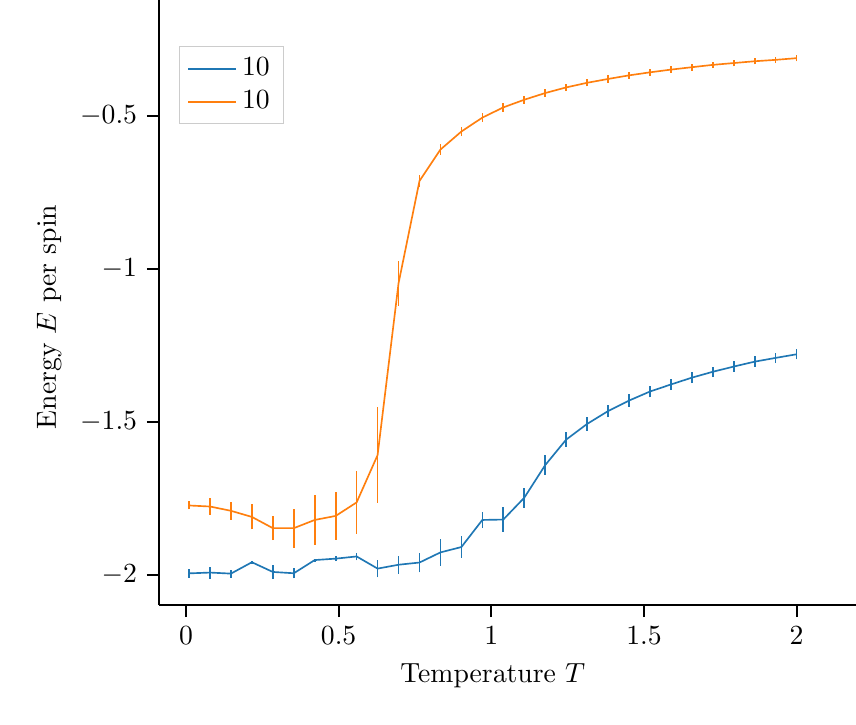
\begin{tikzpicture}

\definecolor{darkgray176}{RGB}{176,176,176}
\definecolor{darkorange25512714}{RGB}{255,127,14}
\definecolor{lightgray204}{RGB}{204,204,204}
\definecolor{steelblue31119180}{RGB}{31,119,180}

\begin{axis}[
legend cell align={left},
legend style={
  fill opacity=0.8,
  draw opacity=1,
  text opacity=1,
  at={(0.03,0.97)},
  anchor=north west,
  draw=lightgray204
},
tick align=outside,
tick pos=left,
x grid style={darkgray176},
xlabel={Temperature \(\displaystyle T\)},
xmin=-0.0895, xmax=2.0995,
xtick style={color=black},
y grid style={darkgray176},
ylabel={Energy \(\displaystyle E\) per spin},
ymin=-2.09902319979481, ymax=-0.214846733941415,
ytick style={color=black}
]
\path [draw=steelblue31119180, semithick]
(axis cs:0.01,-2.00940159517146)
--(axis cs:0.01,-1.98053700898854);

\path [draw=steelblue31119180, semithick]
(axis cs:0.0786206896551724,-2.01206615830345)
--(axis cs:0.0786206896551724,-1.97255869993655);

\path [draw=steelblue31119180, semithick]
(axis cs:0.147241379310345,-2.0087859287851)
--(axis cs:0.147241379310345,-1.9826953875349);

\path [draw=steelblue31119180, semithick]
(axis cs:0.215862068965517,-1.96269947602565)
--(axis cs:0.215862068965517,-1.95439161885435);

\path [draw=steelblue31119180, semithick]
(axis cs:0.28448275862069,-2.0133788149833)
--(axis cs:0.28448275862069,-1.9672730480567);

\path [draw=steelblue31119180, semithick]
(axis cs:0.353103448275862,-2.01102362026044)
--(axis cs:0.353103448275862,-1.97810517397956);

\path [draw=steelblue31119180, semithick]
(axis cs:0.421724137931034,-1.95642239362181)
--(axis cs:0.421724137931034,-1.94641077373819);

\path [draw=steelblue31119180, semithick]
(axis cs:0.490344827586207,-1.95509234848907)
--(axis cs:0.490344827586207,-1.93856055055093);

\path [draw=steelblue31119180, semithick]
(axis cs:0.558965517241379,-1.95244412952991)
--(axis cs:0.558965517241379,-1.92684634183009);

\path [draw=steelblue31119180, semithick]
(axis cs:0.627586206896552,-2.00787321174421)
--(axis cs:0.627586206896552,-1.95082735865579);

\path [draw=steelblue31119180, semithick]
(axis cs:0.696206896551724,-1.99607514880384)
--(axis cs:0.696206896551724,-1.93737911519616);

\path [draw=steelblue31119180, semithick]
(axis cs:0.764827586206897,-1.99208733869643)
--(axis cs:0.764827586206897,-1.92695562370357);

\path [draw=steelblue31119180, semithick]
(axis cs:0.833448275862069,-1.96930870654393)
--(axis cs:0.833448275862069,-1.88345143489607);

\path [draw=steelblue31119180, semithick]
(axis cs:0.902068965517241,-1.94399639218978)
--(axis cs:0.902068965517241,-1.87372839965022);

\path [draw=steelblue31119180, semithick]
(axis cs:0.970689655172414,-1.84665120146144)
--(axis cs:0.970689655172414,-1.79402292445856);

\path [draw=steelblue31119180, semithick]
(axis cs:1.03931034482759,-1.8593794685843)
--(axis cs:1.03931034482759,-1.7786811907757);

\path [draw=steelblue31119180, semithick]
(axis cs:1.10793103448276,-1.78068222462622)
--(axis cs:1.10793103448276,-1.71493306129378);

\path [draw=steelblue31119180, semithick]
(axis cs:1.17655172413793,-1.67309706784008)
--(axis cs:1.17655172413793,-1.60902290223992);

\path [draw=steelblue31119180, semithick]
(axis cs:1.2451724137931,-1.58160008264805)
--(axis cs:1.2451724137931,-1.53389484551195);

\path [draw=steelblue31119180, semithick]
(axis cs:1.31379310344828,-1.52874150433815)
--(axis cs:1.31379310344828,-1.48430522174185);

\path [draw=steelblue31119180, semithick]
(axis cs:1.38241379310345,-1.48479427459037)
--(axis cs:1.38241379310345,-1.44423605708963);

\path [draw=steelblue31119180, semithick]
(axis cs:1.45103448275862,-1.45024455588998)
--(axis cs:1.45103448275862,-1.41011223291002);

\path [draw=steelblue31119180, semithick]
(axis cs:1.51965517241379,-1.42005529211439)
--(axis cs:1.51965517241379,-1.38107419220561);

\path [draw=steelblue31119180, semithick]
(axis cs:1.58827586206897,-1.39604890931988)
--(axis cs:1.58827586206897,-1.35893581228012);

\path [draw=steelblue31119180, semithick]
(axis cs:1.65689655172414,-1.37295550071337)
--(axis cs:1.65689655172414,-1.33750580312663);

\path [draw=steelblue31119180, semithick]
(axis cs:1.72551724137931,-1.35322149902781)
--(axis cs:1.72551724137931,-1.31879512657219);

\path [draw=steelblue31119180, semithick]
(axis cs:1.79413793103448,-1.33579052985162)
--(axis cs:1.79413793103448,-1.30200083590838);

\path [draw=steelblue31119180, semithick]
(axis cs:1.86275862068966,-1.31987105835943)
--(axis cs:1.86275862068966,-1.28592159972057);

\path [draw=steelblue31119180, semithick]
(axis cs:1.93137931034483,-1.30777567147544)
--(axis cs:1.93137931034483,-1.27345731028456);

\path [draw=steelblue31119180, semithick]
(axis cs:2,-1.29532325951322)
--(axis cs:2,-1.26224049360678);

\path [draw=darkorange25512714, semithick]
(axis cs:0.01,-1.78606053584287)
--(axis cs:0.01,-1.76000525191713);

\path [draw=darkorange25512714, semithick]
(axis cs:0.0786206896551724,-1.80311228677963)
--(axis cs:0.0786206896551724,-1.74973973666037);

\path [draw=darkorange25512714, semithick]
(axis cs:0.147241379310345,-1.81918330626443)
--(axis cs:0.147241379310345,-1.76175206885557);

\path [draw=darkorange25512714, semithick]
(axis cs:0.215862068965517,-1.85117515060571)
--(axis cs:0.215862068965517,-1.76970440739429);

\path [draw=darkorange25512714, semithick]
(axis cs:0.28448275862069,-1.88627252085735)
--(axis cs:0.28448275862069,-1.80798781034265);

\path [draw=darkorange25512714, semithick]
(axis cs:0.353103448275862,-1.91107799238211)
--(axis cs:0.353103448275862,-1.78332124553789);

\path [draw=darkorange25512714, semithick]
(axis cs:0.421724137931034,-1.90177833454075)
--(axis cs:0.421724137931034,-1.73889506369925);

\path [draw=darkorange25512714, semithick]
(axis cs:0.490344827586207,-1.88452799961117)
--(axis cs:0.490344827586207,-1.72979172046883);

\path [draw=darkorange25512714, semithick]
(axis cs:0.558965517241379,-1.8648574769578)
--(axis cs:0.558965517241379,-1.6610116048822);

\path [draw=darkorange25512714, semithick]
(axis cs:0.627586206896552,-1.76418205792112)
--(axis cs:0.627586206896552,-1.45235329847888);

\path [draw=darkorange25512714, semithick]
(axis cs:0.696206896551724,-1.12021842301625)
--(axis cs:0.696206896551724,-0.972847966103754);

\path [draw=darkorange25512714, semithick]
(axis cs:0.764827586206897,-0.73236574961624)
--(axis cs:0.764827586206897,-0.69167163006376);

\path [draw=darkorange25512714, semithick]
(axis cs:0.833448275862069,-0.62661217094774)
--(axis cs:0.833448275862069,-0.59270813457226);

\path [draw=darkorange25512714, semithick]
(axis cs:0.902068965517241,-0.566062025690209)
--(axis cs:0.902068965517241,-0.535288838149791);

\path [draw=darkorange25512714, semithick]
(axis cs:0.970689655172414,-0.519107970834819)
--(axis cs:0.970689655172414,-0.491374024765181);

\path [draw=darkorange25512714, semithick]
(axis cs:1.03931034482759,-0.485503696018345)
--(axis cs:1.03931034482759,-0.458181817101655);

\path [draw=darkorange25512714, semithick]
(axis cs:1.10793103448276,-0.459916510894878)
--(axis cs:1.10793103448276,-0.433728776705122);

\path [draw=darkorange25512714, semithick]
(axis cs:1.17655172413793,-0.437479165067947)
--(axis cs:1.17655172413793,-0.412369172372053);

\path [draw=darkorange25512714, semithick]
(axis cs:1.2451724137931,-0.418514483901034)
--(axis cs:1.2451724137931,-0.394547800658966);

\path [draw=darkorange25512714, semithick]
(axis cs:1.31379310344828,-0.403170304467868)
--(axis cs:1.31379310344828,-0.379694590972132);

\path [draw=darkorange25512714, semithick]
(axis cs:1.38241379310345,-0.390499655259397)
--(axis cs:1.38241379310345,-0.367244183540603);

\path [draw=darkorange25512714, semithick]
(axis cs:1.45103448275862,-0.378600006014082)
--(axis cs:1.45103448275862,-0.355714834385918);

\path [draw=darkorange25512714, semithick]
(axis cs:1.51965517241379,-0.36839129602659)
--(axis cs:1.51965517241379,-0.34604471717341);

\path [draw=darkorange25512714, semithick]
(axis cs:1.58827586206897,-0.35927669292776)
--(axis cs:1.58827586206897,-0.33738325579224);

\path [draw=darkorange25512714, semithick]
(axis cs:1.65689655172414,-0.351371610282304)
--(axis cs:1.65689655172414,-0.329601259957696);

\path [draw=darkorange25512714, semithick]
(axis cs:1.72551724137931,-0.343473264452733)
--(axis cs:1.72551724137931,-0.322143550907267);

\path [draw=darkorange25512714, semithick]
(axis cs:1.79413793103448,-0.337556999047295)
--(axis cs:1.79413793103448,-0.316194152792705);

\path [draw=darkorange25512714, semithick]
(axis cs:1.86275862068966,-0.331522904947437)
--(axis cs:1.86275862068966,-0.310428247292563);

\path [draw=darkorange25512714, semithick]
(axis cs:1.93137931034483,-0.326816603104549)
--(axis cs:1.93137931034483,-0.305982922655451);

\path [draw=darkorange25512714, semithick]
(axis cs:2,-0.321308818927067)
--(axis cs:2,-0.300491118752933);

\addplot [semithick, steelblue31119180]
table {%
0.01 -1.99496930208
0.0786206896551724 -1.99231242912
0.147241379310345 -1.99574065816
0.215862068965517 -1.95854554744
0.28448275862069 -1.99032593152
0.353103448275862 -1.99456439712
0.421724137931034 -1.95141658368
0.490344827586207 -1.94682644952
0.558965517241379 -1.93964523568
0.627586206896552 -1.9793502852
0.696206896551724 -1.966727132
0.764827586206897 -1.9595214812
0.833448275862069 -1.92638007072
0.902068965517241 -1.90886239592
0.970689655172414 -1.82033706296
1.03931034482759 -1.81903032968
1.10793103448276 -1.74780764296
1.17655172413793 -1.64105998504
1.2451724137931 -1.55774746408
1.31379310344828 -1.50652336304
1.38241379310345 -1.46451516584
1.45103448275862 -1.4301783944
1.51965517241379 -1.40056474216
1.58827586206897 -1.3774923608
1.65689655172414 -1.35523065192
1.72551724137931 -1.3360083128
1.79413793103448 -1.31889568288
1.86275862068966 -1.30289632904
1.93137931034483 -1.29061649088
2 -1.27878187656
};
\addlegendentry{10}
\addplot [semithick, darkorange25512714]
table {%
0.01 -1.77303289388
0.0786206896551724 -1.77642601172
0.147241379310345 -1.79046768756
0.215862068965517 -1.810439779
0.28448275862069 -1.8471301656
0.353103448275862 -1.84719961896
0.421724137931034 -1.82033669912
0.490344827586207 -1.80715986004
0.558965517241379 -1.76293454092
0.627586206896552 -1.6082676782
0.696206896551724 -1.04653319456
0.764827586206897 -0.71201868984
0.833448275862069 -0.60966015276
0.902068965517241 -0.55067543192
0.970689655172414 -0.5052409978
1.03931034482759 -0.47184275656
1.10793103448276 -0.4468226438
1.17655172413793 -0.42492416872
1.2451724137931 -0.40653114228
1.31379310344828 -0.39143244772
1.38241379310345 -0.3788719194
1.45103448275862 -0.3671574202
1.51965517241379 -0.3572180066
1.58827586206897 -0.34832997436
1.65689655172414 -0.34048643512
1.72551724137931 -0.33280840768
1.79413793103448 -0.32687557592
1.86275862068966 -0.32097557612
1.93137931034483 -0.31639976288
2 -0.31089996884
};
\addlegendentry{10}
\end{axis}

\end{tikzpicture}

\caption{}
\label{fi:energies_T_q_L50}
\end{minipage}
\end{figure}

In figure \ref{fi:t0_T_q_L50} one sees the number of iterations $t_0$ it took the simulation to reach an equilibrium.
For this it takes the simulation in most cases roughly $0.25\cdot 10^7$ steps. However, for cold temperatures with $q=10$ this takes far longer since the system starts in the `hot' state similar to the state previously depicted in figure \ref{fi:High_temp_state} and must first reach the `cold' state.

\begin{figure}
\centering
\begin{minipage}{0.7\textwidth}
\centering
\graphicspath{{../../Plots/}}
% This file was created with tikzplotlib v0.10.1.
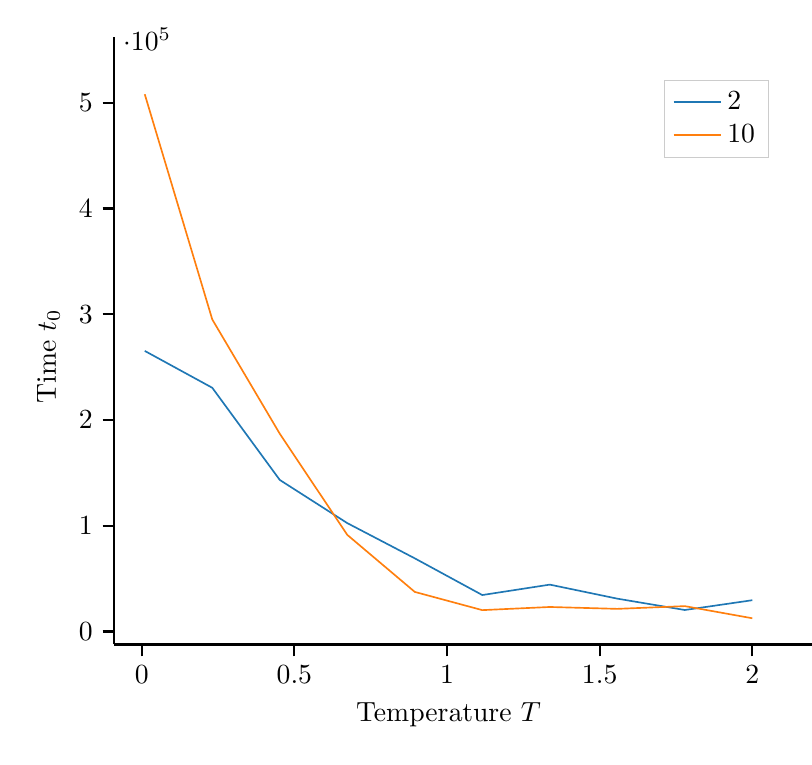
\begin{tikzpicture}

\definecolor{darkgray176}{RGB}{176,176,176}
\definecolor{darkorange25512714}{RGB}{255,127,14}
\definecolor{lightgray204}{RGB}{204,204,204}
\definecolor{steelblue31119180}{RGB}{31,119,180}

\begin{axis}[
legend cell align={left},
legend style={fill opacity=0.8, draw opacity=1, text opacity=1, draw=lightgray204},
tick align=outside,
tick pos=left,
x grid style={darkgray176},
xlabel={Temperature \(\displaystyle T\)},
xmin=-0.0895, xmax=2.0995,
xtick style={color=black},
y grid style={darkgray176},
ylabel={Time \(\displaystyle t_0\)},
ymin=-12185.65, ymax=532878.65,
ytick style={color=black}
]
\addplot [semithick, steelblue31119180]
table {%
0.01 265401
0.231111111111111 230543
0.452222222222222 143393
0.673333333333333 102574
0.894444444444444 69257
1.11555555555556 34553
1.33666666666667 44411
1.55777777777778 31140
1.77888888888889 20403
2 29668
};
\addlegendentry{2}
\addplot [semithick, darkorange25512714]
table {%
0.01 508103
0.231111111111111 295154
0.452222222222222 187078
0.673333333333333 91453
0.894444444444444 37511
1.11555555555556 20291
1.33666666666667 23267
1.55777777777778 21487
1.77888888888889 24068
2 12590
};
\addlegendentry{10}
\end{axis}

\end{tikzpicture}

\caption{Time $t_0$ until the equilibrium is reached.}
\label{fi:t0_T_q_L50}
\end{minipage}
\end{figure}

In another series of experiments we wanted to see how the energy dependence of the temperature depends on the system size $L$. The results are shown in figures \ref{fi:energies_T_q_L5} and \ref{fi:energies_T_q_L10} for system sizes $L=5$ and $L=10$ respectively. Both look quite similar to the case $L=50$. One notices that as the state size $L$ decreases the standard deviation for the energies per spin increases. This is probably due to the fact that in a smaller system a change of some spins and thus a change of energy is has a greater impact in relation to the total energy of the system.
It is also noticeable that the curve for the parameter $q=10$ smooths out as the system size decreases.

\begin{figure}
\centering
\begin{minipage}{0.7\textwidth}
\centering
\graphicspath{{../../Plots/}}
\input{../../Plots/energies_T_q_L5.pgf}
\caption{$L=5$.}
\label{fi:energies_T_q_L5}
\end{minipage}
\end{figure}

\begin{figure}
\centering
\begin{minipage}{0.7\textwidth}
\centering
\graphicspath{{../../Plots/}}
\input{../../Plots/energies_T_q_L10.pgf}
\caption{$L=10$.}
\label{fi:energies_T_q_L10}
\end{minipage}
\end{figure}


\subsection{Plotting the energy distribution around the Curie temperature}

In a final experiment we plotted the distribution of energies around the Curie temperature for a grid size of $L=50$ and parameter $q=10$. The number of sampling steps was chosen as \pyth{M_sampling=10E7}. In figure \ref{fi:T0697} we see that the distribution of energies splits up at the temperature $T=0.697$. In figures \ref{fi:T0696} and \ref{fi:T0698} the distribution lies around the energy $-1$ for the slightly different temperatures $T=0.696$ and $T=0.698$. For the slightly lower temperature $T=0.695$ in \ref{fi:T0695} the distribution hovers around the significantly lower energy value of $-1.7$.
This is characteristic behaviour for the instability of the system around the Curie temperature. 

%\begin{figure}
%\centering
%\begin{minipage}{0.7\textwidth}
%\centering
%\graphicspath{{../../Plots/}}
%\input{../../Plots/Energies_maxwell_distribution_MC_step_fast_T0.697_3.pgf}
%\caption{Distribution of energies for the temperature $T=0.697$.}
%\label{fi:T0697}
%\end{minipage}
%\end{figure}

%\begin{figure}
%\centering
%\begin{minipage}{0.7\textwidth}
%\centering
%\graphicspath{{../../Plots/}}
%\input{../../Plots/Energies_evolution_MC_step_fast_T0.697_M100000000.pgf}
%\caption{Energy evolution of energies for the temperature $T=0.698$.}
%\label{fi:T0697}
%\end{minipage}
%\end{figure}

\begin{figure}
\centering
\begin{minipage}[b]{0.45\textwidth}
\centering
\graphicspath{{../../Plots/}}
\input{../../Plots/Energies_maxwell_distribution_MC_step_fast_T0.695_3.pgf}
\caption{Distribution of energies for the temperature  $T=0.695$.}
\label{fi:T0695}
\end{minipage}
\hfill
\begin{minipage}[b]{0.45\textwidth}
\centering
\graphicspath{{../../Plots/}}
\input{../../Plots/Energies_maxwell_distribution_MC_step_fast_T0.696_3.pgf}
\caption{Distribution of energies for the temperature  $T=0.696$.}
\label{fi:T0696}
\end{minipage}
\end{figure}

\begin{figure}
\centering
\begin{minipage}[b]{0.45\textwidth}
\centering
\graphicspath{{../../Plots/}}
\input{../../Plots/Energies_maxwell_distribution_MC_step_fast_T0.697_3.pgf}
\caption{Distribution of energies for the temperature  $T=0.697$.}
\label{fi:T0697}
\end{minipage}
\hfill
\begin{minipage}[b]{0.45\textwidth}
\centering
\graphicspath{{../../Plots/}}
\input{../../Plots/Energies_maxwell_distribution_MC_step_fast_T0.698_3.pgf}
\caption{Distribution of energies for the temperature  $T=0.698$.}
\label{fi:T0698}
\end{minipage}
\end{figure}

\section{Conclusion}


We have seen that one can use the Metropolis Monte-Carlo and the heat-bath algorithm to effectively simulate the Potts model. Both algorithms yield consistent results for different initial values and 
the distribution of energy approximates a distribution similar to the Maxwell-Boltzmann distribution. 
We also saw that the energy for the parameter $q=10$ jumped around the Curie temperature. This jump became more pronounced for increased system size. We also saw this jump when plotting the distribution of the energy for a temperature around the Curie temperature. In the case of $q=2$ the energy on the other hand increased gradually with increasing temperature.
We have seen in the project that the number of steps a simulation is able to run for is critical for the ability to produce meaningful results. Here we discovered the efficiency of the code played a crucial role.

\newpage
\section*{Bibliography}
\nocite{*}
%Main source
%\printbibliography[heading=none, keyword={main}]
%\noindent Other sources
\printbibliography[heading=none, keyword={secondary}]


\end{document}
